\documentclass{beamer}
\beamertemplatenavigationsymbolsempty
\usecolortheme{beaver}
\setbeamertemplate{blocks}[rounded=true, shadow=true]
\setbeamertemplate{footline}[page number]
%
\usepackage[utf8]{inputenc}
\usepackage[english, russian]{babel}
\usepackage{amssymb,amsfonts,amsmath,mathtext}
\usepackage{subfig}
\usepackage{booktabs}
\usepackage[all]{xy} % xy package for diagrams
\usepackage{array}
\usepackage{multicol}% many columns in slide
\usepackage{hyperref}% urls
\usepackage{hhline}%tables
% Your figures are here:
\graphicspath{ {fig/} {../fig/} }

%----------------------------------------------------------------------------------------------------------
\title[\hbox to 56mm{Генерация}]{Применение синтетических данных, полученных с помощью генеративной нейросети, для повышения качества моделей детекции}
\author[N.\,P.~Ivkin]{Степанов Илья}
\institute{Московский физико-технический институт}
\date{\footnotesize
\par\smallskip\emph{Курс:} НИР
\par\smallskip\emph{Научный руководитель:} Грабовой Андрей Валерьевич
\par\smallskip\emph{Консультант:} Филатов Андрей Викторович
\par\bigskip\small 2024}

%----------------------------------------------------------------------------------------------------------
\begin{document}
%----------------------------------------------------------------------------------------------------------
\begin{frame}
\thispagestyle{empty}
\maketitle
\end{frame}
%-----------------------------------------------------------------------------------------------------
\begin{frame}{Цель исследования}


\textbf{Задача} 

Создание высококачественных аугментаций с использованием генеративной нейросети для повышения качества моделей детекции.

\vspace{5pt} % добавляем дополнительное пространство

\textbf{Проблема} 

Существующие методы аугментации с применением генеративных нейросетей обладают рядом недостатков, таких как: невозможность генерировать новые классы объектов; отсутствие физичности у синтетических изображений.

\vspace{5pt} % добавляем дополнительное пространство

\textbf{Цель} 

Создание автоматизированного pipeline, способного качественно генерировать аугментации, нивелируя проблемы предыдущих подходов. Проведение сравнений аугментаций на датасетах COCO и Pascal VOC с использованием моделей детекции, а также проведение ablation.

\end{frame}
%------------------------------------------------------------------------------------------
\begin{frame}{Постановка задачи}

{\small Определим датасет как $ \mathfrak{D}=\{ {x}_{i}: i = 1, \dots, n\}$, ${x}_{i}$ --- изображение. Рассматривается диффузионная модель для аугментации $\epsilon_{\theta}$. Определим функцию потерь:
\begin{center}
    $\mathcal{L}(\epsilon, \epsilon_{\theta}) = \mathbb{E}_{\epsilon \sim N(0, I), m_i, \tau_i, \tilde{x_i}, t} \|\epsilon - \epsilon_{\theta}(x^t_i, m_i,\tau_i, \tilde{x_i}, t)\|^2,$
\end{center}
где $x^t_i$ -- зашумленное изображение на шаге $t$, $m_i$ -- сегментационная маска данного изображения, $\tau_i$ -- текстовая подсказка данного изображения,
$\tilde{x_i}$ = $(1 - m_i) \ \odot x_i$, $t \in [0, T]$ -- шаг диффузионного процесса. Для получения масок и текстовых подсказок мы используем модели сегментации и "image-to-text".
% Модифицированный датасет после аугментаций определим как $\tilde{\mathfrak{D}} = \{ \phi_{\theta}({x}_{i}): i = 1, \dots, n\}$, ${x}_{i}$ --- изображение. Требуется оценить качество синтетических данных $\tilde{\mathfrak{D}}$, используя модели детекции.
}

\end{frame}
%------------------------------------------------------------------------------------------

\begin{frame}{Архитектура модели}

\begin{figure}[!t]
    \centering
    \includegraphics[width=1\textwidth]{aug_garage.pdf}
\end{figure}

\scriptsize
На рисунке изображён автоматический pipeline. Модель принимает изображение, после чего процесс аугментации разделён на следующие этапы:

\begin{itemize} \item Подготовка к аугментации начинается с генерации описания изображения с помощью модели LLaVA. Далее модель SAM генерирует маску для случайного объекта, после чего модель LLaMA использует эту маску и описание изображения для создания расширенной подсказки. \item Расширенная подсказка, маска и исходное изображение подаются в модель PowerPaint, которая генерирует аугментацию. \item На этапе постобработки проводится фильтрация с использованием AlphaCLIP, а также уточняется маска сгенерированного объекта при помощи SAM. \end{itemize}

\end{frame}

\begin{frame}{Эксперименты}

\begin{figure}[!t]
    \centering
    \includegraphics[width=1\textwidth]{1.jpeg}
\end{figure}

\scriptsize
В таблице записаны результаты детекции объектов на наборе данных Pascal VOC. Обучение на наших данных значительно улучшает производительность моделей детекции, что подтверждается более высокими значениями AP в строках "наши" по сравнению с "оригинальные". Проценты представляют собой долю изображений с кошками, использованных из оригинального набора данных.

\end{frame}

\begin{frame}{Эксперименты}

\begin{figure}[!t]
    \centering
    \begin{minipage}{0.48\textwidth}
        \centering
        \includegraphics[width=\textwidth]{2.jpeg}
    \end{minipage} \hfill
    \begin{minipage}{0.48\textwidth}
        \centering
        \includegraphics[width=\textwidth]{3.jpeg}
    \end{minipage}
\end{figure}

\scriptsize
 В таблице записаны результаты сравнения качества обучения модели FasterRCNN в зависимости от расширения подсказки. Результаты показывают, что использование расширенных подсказок значительно повышает AP для категории "кошка" по сравнению с использованием обычных инструкций. На картинке продемонстрирована генерация с помощью разных подсказок.


\end{frame}

\begin{frame}{Эксперименты}

\begin{figure}[!t]
    \centering
    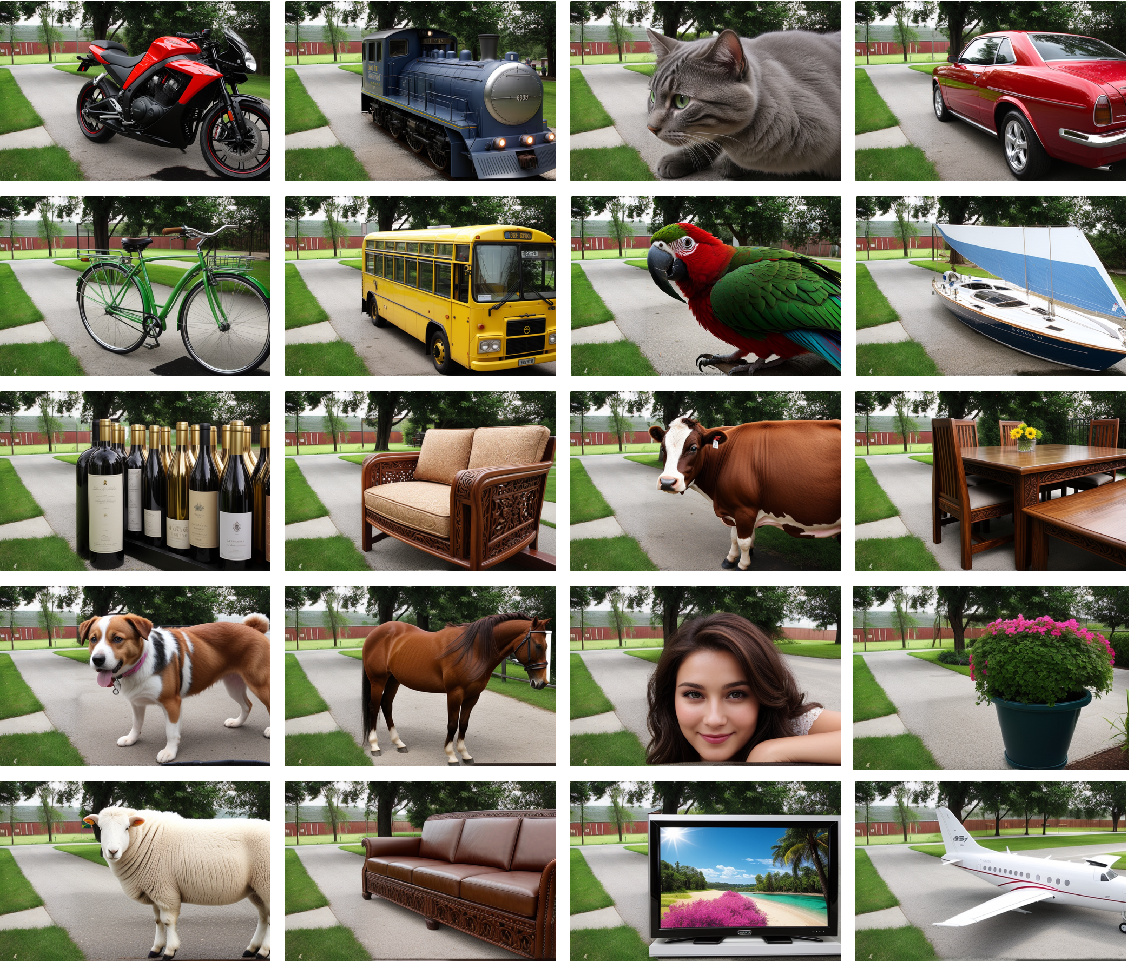
\includegraphics[width=0.7\textwidth]{generation_examples.pdf}
\end{figure}

\scriptsize На картинке продемонстрированы результаты генераций с помощью нашего подхода.


\end{frame}

%------------------------------------------------------------------------------------------

%------------------------------------------------------------------------------------------

%------------------------------------------------------------------------------------------
\begin{frame}{План работы на следующий семестр}

\begin{itemize}
    \item  Собрать автоматический pipeline
    \item  Сделать сравнение с существующими методами на датасетах Coco и Pascal VOC
    \item  Провести ablation модели
\end{itemize}

\end{frame}
%---------------------------------------------------------------------------------------
%----------------------------------------------------------------------------------------------------------
\end{document} 